\documentclass{tufte-handout}

\usepackage{style}

\begin{document}

\documentclass[tikz,border=5mm]{standalone}
\usepackage{tikz}
\usetikzlibrary{calc,arrows.meta}

\begin{document}
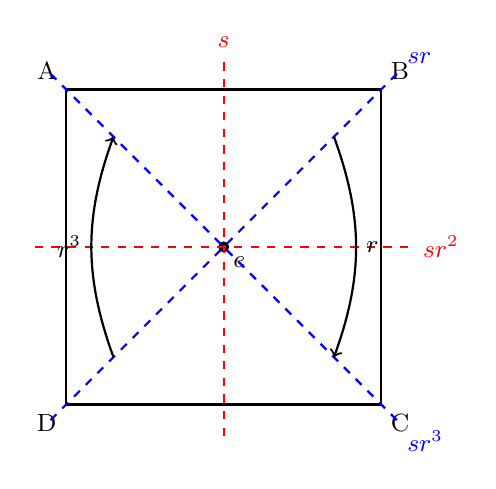
\begin{tikzpicture}[scale=2, every node/.style={font=\small}]
    % Define corners of square
    \coordinate (A) at (-1,1);
    \coordinate (B) at (1,1);
    \coordinate (C) at (1,-1);
    \coordinate (D) at (-1,-1);

    % Draw square
    \draw[thick] (A)--(B)--(C)--(D)--cycle;
    \node[above left] at (A) {A};
    \node[above right] at (B) {B};
    \node[below right] at (C) {C};
    \node[below left] at (D) {D};

    % Rotation center
    \fill (0,0) circle (1pt) node[below right] {$e$};

    % Reflection axes
    % vertical (s)
    \draw[red, thick, dashed] (0,-1.2) -- (0,1.2) node[above] {$s$};
    % horizontal (sr^2)
    \draw[red, thick, dashed] (-1.2,0) -- (1.2,0) node[right] {$sr^2$};
    % diagonal 1 (sr)
    \draw[blue, thick, dashed] (-1.1,-1.1) -- (1.1,1.1) node[above right] {$sr$};
    % diagonal 2 (sr^3)
    \draw[blue, thick, dashed] (-1.1,1.1) -- (1.1,-1.1) node[below right] {$sr^3$};

    % Rotation arrows
    \draw[thick, ->, bend left=20] (0.7,0.7) to node[right] {$r$} (0.7,-0.7);
    \draw[thick, ->, bend left=20] (-0.7,-0.7) to node[left] {$r^3$} (-0.7,0.7);
\end{tikzpicture}
\end{document}



\end{document}